%----------------------------------------------------------------------
\begin{frame}[c]{Where are we? The big picture}

\begin{itemize}
\item[$\to$] Algorithm Selection
  \begin{itemize}
    \item Portfolios
    \item[$\to$] Algorithm selection (focus on runtime)
  \end{itemize}
  \item Design Decisions:\\ Local Search + Evo. Algorithms + Machine Learning 
  \item Empirical evaluation
  \item AAD for ML
  \begin{itemize}
    \item Hyperparameter optimization and Bayesian Optimization 
    \item Neural architecture search (lecture given by Prof. Hutter)
  \end{itemize}
  \item Algorithm configuration 
  \begin{itemize}
    \item Basics 
    \item State of the art 
    \item Best Practices 
  \end{itemize}
  \item Combinations of algorithm selection and configurations
  \item Algorithm control 
  \item Algorithm analysis 
  \item Project announcement and questions for exam 
\end{itemize}

\end{frame}
%----------------------------------------------------------------------
%----------------------------------------------------------------------
\begin{frame}[c, fragile]{}

\centering
{\huge
State-of-the-art Algorithm Selection
}

\bigskip
\bigskip
\bigskip

\scalebox{0.8}{
\tikzstyle{activity}=[rectangle, draw=black, rounded corners, text centered, text width=8em, fill=white, drop shadow]
\tikzstyle{data}=[rectangle, draw=black, text centered, fill=black!10, text width=8em, drop shadow]
\tikzstyle{myarrow}=[->, thick]
\begin{tikzpicture}[align=center,node distance=3.7cm, thick]
	%PreProcessing
	%\node (PreSolving) [activity, right of=Instance] {Run Pre-Solving Schedule};
	\node (Features) [activity] {Compute\\ Features $\feat(\inst)$};
	\node (Instance) [data, left of=Features] {Instance $\inst$};
	\node (Select) [activity, right of=Features] {Select Algorithm\\ $\feat(\inst) \mapsto \hat{a}$};
	\node (Solve) [activity, right of=Select] {Run $\hat{a}$ on $\inst$};
	\node (Portfolio) [data, above of=Select, yshift=-2.0cm] {Algorithm Portfolio $\portfolio$};

	\draw[myarrow] (Instance) -- (Features);
	%\draw[myarrow] (PreSolving) -- (Features);
	\draw[myarrow] (Features) -- (Select);
	\draw[myarrow] (Select) -- (Solve);
	\draw[myarrow] (Portfolio) -- (Select);
	%\draw[myarrow] (Portfolio) -- (PreSolving);

\end{tikzpicture}
}

\end{frame}
%----------------------------------------------------------------------
%----------------------------------------------------------------------
\begin{frame}[c]{Learning Goals}

After this lecture, you will be able to \ldots

\begin{itemize}
  \item explain all components of \alert{\satzilla}
  \item explain other algorithm selection approaches
  \begin{itemize}
	  \item \alert{pair-wise regression} 
	  \item \alert{cost-sensitive classification} 
	  \item \alert{clustering} 
	  \item \alert{kNN}
	  \item \alert{per-instance algorithm schedules}
  \end{itemize}
  \item describe a \alert{flexible framework} for algorithm selection
  \item decide \alert{when} to use algorithm selection
  %\item combine of \alert{algorithm selection and configuration}
\end{itemize}
\end{frame}
%-----------------------------------------------------------------------
%----------------------------------------------------------------------
\begin{frame}[c]{\satzilla{}~\litw{Xu et al. 2009}}

\begin{enumerate}
	\item use a static algorithm schedule (called pre-solving schedule)
	\item if pre-solving schedule failed, compute instance features 
	\item run algorithm with best predicted performance
	  \begin{itemize}
	    \item use regression models to predict performance of each algorithm\\
	  \end{itemize}
\end{enumerate}

\centering
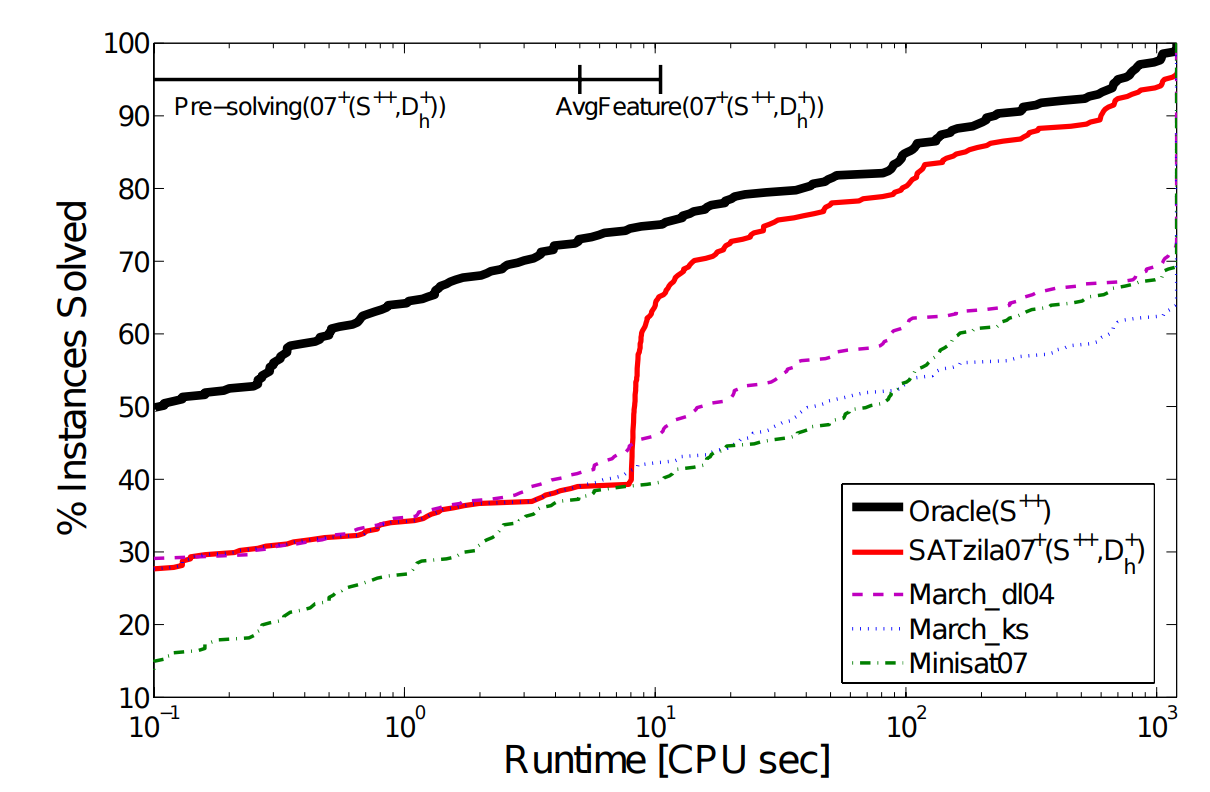
\includegraphics[width=0.8\textwidth]{images/satzilla}

\end{frame}
%-----------------------------------------------------------------------
% %----------------------------------------------------------------------
% \begin{frame}[c]{Empirical Performance Model: EPM}
% 
% \centering
% $\feats \to \perf$
% 
% \begin{center}
% \vspace*{-1em}
% \includegraphics[width=0.6\textwidth]{images/regression}
% \end{center}
% \tiny
% 
% \vspace*{-4em}
% (Source: \url{http://scikit-learn.org/})
% 
% \end{frame}
% %-----------------------------------------------------------------------
%----------------------------------------------------------------------
\begin{frame}[c]{\satzilla{} - Training}

\begin{enumerate}
  \item Identify target set of \alert{problem instances} 
  \begin{itemize}
    \item representative of some underlying distribution
  \end{itemize}
  \item Select a \alert{portfolio} of candidate algorithms
  \begin{itemize}
    \item complementary!
    \item each algorithm performs well on at least some instances
  \end{itemize}
  \pause
  \medskip
  \item Identify \alert{instance features} that characterize problem instances
  \item On a training set of problem instances, compute these \alert{features} and run each algorithm to determine its \alert{runtimes}
  \pause
  \medskip
  \item Identify one or more algorithms for \alert{pre-solving} ($\to$ schedule)
  \begin{itemize}
    \item e.g., brute force search on a discretized set of runtimes
  \end{itemize} 
  %\item Identify the single best algorithm
  \pause
  \medskip
  \item Train \alert{regression model} for each algorithm: $\feats \to \perf$
  \item Choose the \alert{best subset of algorithms} to use in the final portfolio
\end{enumerate}

\end{frame}
%-----------------------------------------------------------------------
% %----------------------------------------------------------------------
% \begin{frame}[c]{\satzilla{} - Selection}
% 
% \begin{enumerate}
%   \item Run pre-solving schedule
%   \item Compute feature values; if it fails, select the backup algorithm
%   \item Otherwise, predict each algorithm's runtime using the EPM
%   \item Run the algorithm predicted to be the best\\ (If an algorithm fails to complete its run (e.g., it crashed), run the algorithm predicted to be next best.)
% \end{enumerate}
% 
% \scalebox{0.6}{
% \tikzstyle{activity}=[rectangle, draw=black, rounded corners, text centered, text width=8em, fill=white, drop shadow]
\tikzstyle{data}=[rectangle, draw=black, text centered, fill=black!10, text width=8em, drop shadow]
\tikzstyle{myarrow}=[->, thick]
\begin{tikzpicture}[align=center,node distance=3.7cm, thick]
	%PreProcessing
	\node (Instance) [data] {Instance $\inst$};
	\node (PreSolving) [activity, right of=Instance] {Run Pre-Solving Schedule};
	\node (Features) [activity, right of=PreSolving] {Compute\\ Features $\feat(\inst)$};
	\node (Backup) [activity, below of=Features, yshift=2.0cm] {Backup solver};
	\node (Select) [activity, right of=Features] {Select Algorithm\\ $\feat(\inst) \mapsto \hat{a}$};
	\node (Solve) [activity, right of=Select] {Run $\hat{a}$ on $\inst$};
	\node (Portfolio) [data, above of=Select, yshift=-2.0cm] {Algorithm Portfolio $\portfolio$};

	\draw[myarrow] (Instance) -- (PreSolving);
	\draw[myarrow] (PreSolving) -- (Features);
	\draw[myarrow] (Features) -- (Select);
	\draw[myarrow] (Features) -- (Backup);
	\draw[myarrow] (Select) -- (Solve);
	\draw[myarrow] (Portfolio) -- (Select);
	%\draw[myarrow] (Portfolio) -- (PreSolving);

\end{tikzpicture}
% }
% 
% \end{frame}
% %-----------------------------------------------------------------------
% %----------------------------------------------------------------------
% \begin{frame}[c]{Prediction of runtimes: Ridge regression}
% 
% \begin{itemize}
%   \item Set of feature vectors $\feat(\inst)$ that characterizes the instances $\inst \in \insts$
%   \item Measured log-runtime $y_{\algo, \inst} = \log t(\algo, \inst)$ 
%   \pause
%   \medskip
%   \item Ridge regression suffers from highly correlated and uninformative features\\ $\to$ use forward feature selection
%   \item Add quadratic basis features $\feat_{j}(\inst) \cdot \feat_{k}(\inst)$ for $j \in \{1 \ldots m\}$ and $k = \{j \ldots m \}$; use another pass of forward feature selection\\
%   		$\to$ $\vec{\phi}_{\inst} = \vec{\phi(\feat(\inst))}$
%   \pause
%   \item Let $\Phi$ be an $n \times d$ matrix for $n$ training instances and $d$ final features of basis function
%   \item $\vec{w} = (\delta I + \Phi^\intercal\Phi)^{-1}\Phi^\intercal\vec{y}$ with $I$ being the identity matrix and $\delta$ being a small constant to penalize large coefficients $\vec{w}$ (e.g., $\delta=10^{-3}$)
%   \pause
%   \medskip
%   \item $f_{\vec{w}}(\feat(\inst)) = \vec{w}^\intercal \phi(\feat(\inst))$
% \end{itemize}
% 
% \end{frame}
% %-----------------------------------------------------------------------
%----------------------------------------------------------------------
\begin{frame}[c]{Accounting for Censored Data}

\begin{block}{Problem}
The measured runtimes $t(\algo, \inst)$ can include timeouts and memouts,\\
i.e., left-censored data: we know only a lower bound on the true runtime.
\end{block}

\bigskip
\pause

\begin{block}{Solution~\litw{Schmee and Hahn 1979}}
Repeat until convergence:
\begin{enumerate}
  \item Estimate the expected runtime of censored runs using regression models (under consideration of censoring)
  \item Train a new regression model using true runtimes for the uncensored instances and the
predictions generated in the previous step for the censored instances.
\end{enumerate}
\end{block}


\end{frame}
%-----------------------------------------------------------------------
%----------------------------------------------------------------------
\begin{frame}[c]{Handling of Censored Data\litw{Schmee and Hahn 1979}}

\begin{block}{Censored Data}
\begin{itemize}
  \item Only lower bound of cost is known
  \item Censoring can be at different lower bounds
\end{itemize}
\end{block}

\pause

\begin{algorithm}[H]
\Input{Uncensored data $\mathbf{X}_{\text{u}}, \mathbf{y}_{\text{u}}$, Censored data $\mathbf{X}_{\text{c}}, \mathbf{y}_{\text{c}}$}
\Output{Imputed values $y_{\text{imp}}$ for $\mathbf{X}_{\text{c}}$}
\BlankLine
model.fit($\mathbf{X}_{\text{u}}, \mathbf{y}_{\text{u}}$);\\
\While{not converged} {
	\ForEach{censored sample $i$} {
		$\mu,\sigma^2$ := model.predict($\mathbf{X}_{\text{c}}^{(i)}$);\\
		$\mathbf{y}_{\text{imp}}^{(i)}$ := mean of $\mathcal{N}(\mu, \sigma^2)_{\geq \mathbf{y}_{\text{c}}^{(i)}}$;\\
	}
	model.fit($\mathbf{X}_{\text{u}} || \mathbf{X}_{\text{c}}, \mathbf{y}_{\text{u}} || \mathbf{y}_{\text{imp}}$);\\
}
\Return{$\mathbf{y}_{\text{imp}}$}
\end{algorithm}

\end{frame}
%-----------------------------------------------------------------------
%----------------------------------------------------------------------
\begin{frame}[c]{Hierarchical Performance Models}

\begin{block}{Observations}
\begin{itemize}
  \item A set of CNFs consists of satisfiable (SAT: NP-problem) and unsatisfiable instances (UNSAT: co-NP-problem).
  \item SAT and UNSAT instances have different performance characteristics
  \item How to know whether an instance belongs to SAT or UNSAT?
\end{itemize}
\end{block}

\pause

\begin{block}{Solution}
\begin{itemize}
  \item Use machine learning to predict the probability of\\ being SAT or UNSAT
  \item Learn different performance models for SAT and UNSAT instances
\end{itemize}

\begin{equation}
P(y_\inst|\feat(\inst)) = \sum_{k\in \{SAT,UNSAT\}} P(z=k | \feat(\inst)) \cdot P_{M_k} (y | \feat(\inst))) \nonumber
\end{equation}

\end{block}

$\leadsto$ \alert{Hierarchical models can be used to improve performance!}

\end{frame}
%-----------------------------------------------------------------------
%----------------------------------------------------------------------
\begin{frame}[c]{RTD of \satzilla{} on Random Instances}

\centering
\includegraphics[width=0.8\textwidth]{images/rtd_satzilla_random.png}

\end{frame}
%-----------------------------------------------------------------------
%----------------------------------------------------------------------
\begin{frame}[c]{RTD of \satzilla{} on Industrial Instances}

\centering
\includegraphics[width=0.8\textwidth]{images/rtd_satzilla_indu.png}

\end{frame}
%-----------------------------------------------------------------------
%----------------------------------------------------------------------
\begin{frame}[c]{Further Algorithm Selection Approaches}

\centering
What could be other approaches for algorithm selection?

\bigskip

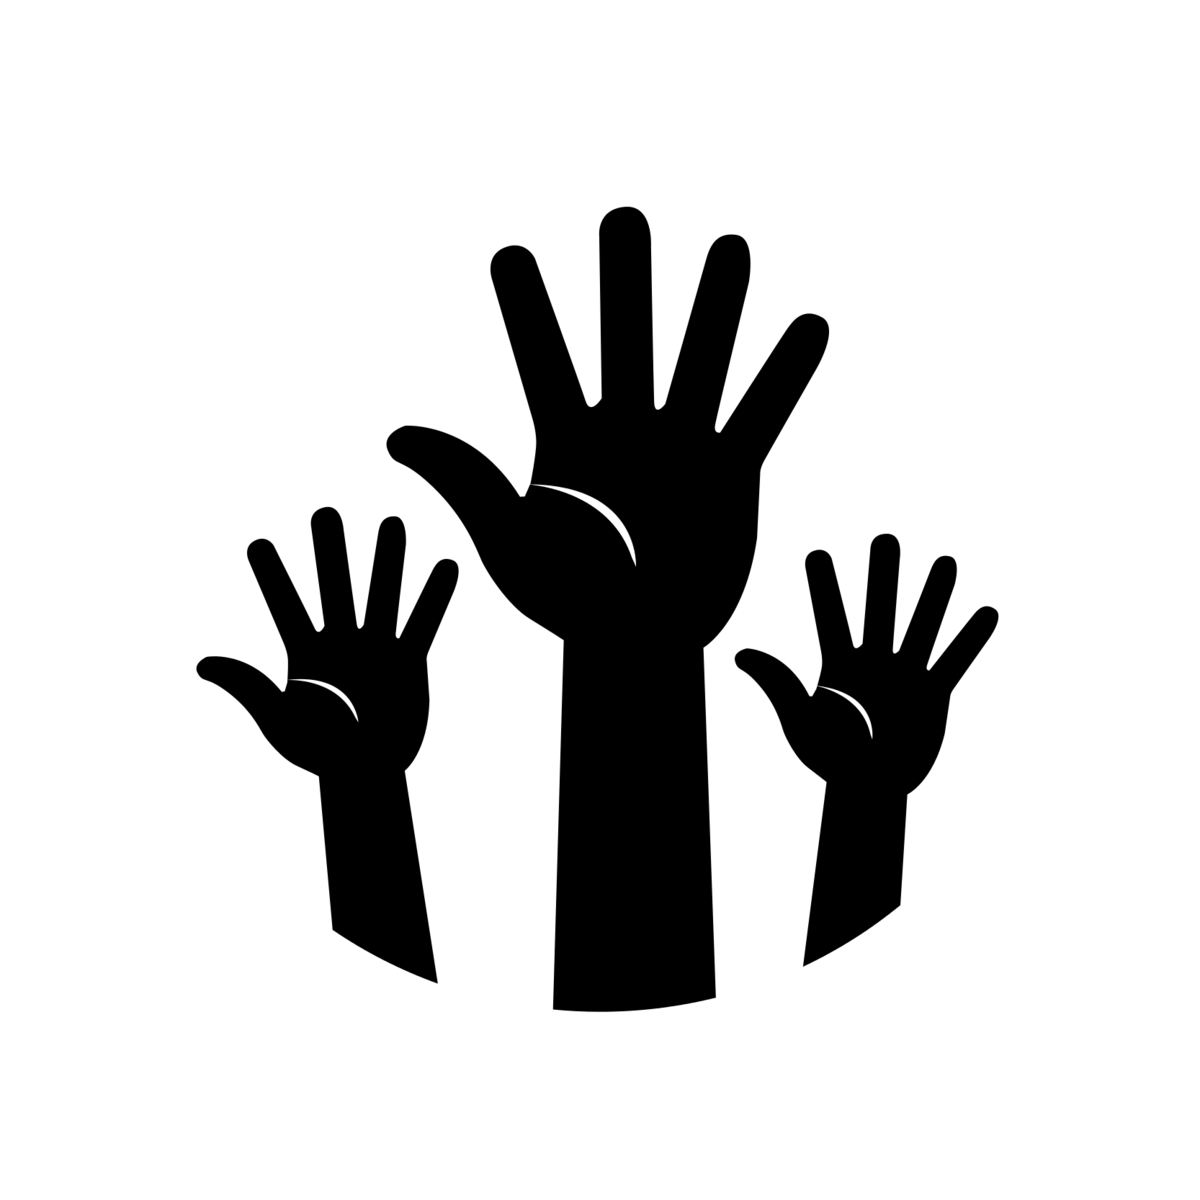
\includegraphics[width=0.2\textwidth]{images/hands.png}

\end{frame}
%-----------------------------------------------------------------------

%----------------------------------------------------------------------
\begin{frame}[c]{Algorithm Selection~\litw{Rice 1976}}

\begin{block}{Definition}
Given 
\begin{itemize}
  \item a set $\insts$ of problem instances,
  \item a portfolio of algorithms $\portfolio$,
  \item and a cost metric $c:  \portfolio \times \insts \rightarrow \perf$,   
\end{itemize}
 
the \emph{per-instance algorithm selection problem} is to find a mapping 
$s: \insts \rightarrow \portfolio$ 
that optimizes $\sum_{\inst \in \insts} c(s(\inst),\inst)$, 
the sum of performance measures achieved by running the selected algorithm $s(\inst)$ for instance~$\inst$.
\end{block}

\bigskip
\pause

$\leadsto$ \alert{That's actually a multiclass classification problem\\ and not a regression problem!}

\end{frame}
%-----------------------------------------------------------------------

%----------------------------------------------------------------------
\begin{frame}[c]{Multiclass Classification}

\begin{block}{Multiclass Classification}
\begin{itemize}
  \item Classes are mutually exclusive
  \begin{itemize}
    \item either observation belongs to class A, B or C
  \end{itemize}
  \item Generalization of binary classification
  \begin{itemize}
    \item approaches map multiclass problem back to binary-class problem:
    \item I: one-vs-rest
    \item II: one-vs-one
  \end{itemize}
\end{itemize}
\end{block}

\end{frame}
%-----------------------------------------------------------------------
%----------------------------------------------------------------------
\begin{frame}[c]{Multiclass Classification: One-vs-Rest}

\includegraphics[width=0.9\textwidth]{images/one_vs_rest}

\end{frame}
%-----------------------------------------------------------------------
%----------------------------------------------------------------------
\begin{frame}[c]{Multiclass Classification: One-vs-One}

\includegraphics[width=0.9\textwidth]{images/one_vs_one}

\end{frame}
%-----------------------------------------------------------------------
%----------------------------------------------------------------------
\begin{frame}[c]{Algorithm Selection~\litw{Rice 1976}}

\begin{block}{Definition}
Given 
\begin{itemize}
  \item a set $\insts$ of problem instances,
  \item a portfolio of algorithms $\portfolio$,
  \item and a cost metric $c:  \portfolio \times \insts \rightarrow \perf$,   
\end{itemize}
 
the \emph{per-instance algorithm selection problem} is to find a mapping 
$s: \insts \rightarrow \portfolio$ 
that optimizes $\sum_{\inst \in \insts} m(s(\inst),\inst)$, 
the sum of performance measures achieved by running the selected algorithm $s(\inst)$ for instance~$\inst$.
\end{block}

\bigskip
\pause

$\leadsto$ \alert{Not quite a multiclass classification problem,\\ because of a special loss function for each instance.}

\end{frame}
%-----------------------------------------------------------------------


%----------------------------------------------------------------------
\begin{frame}[c]{\satzillaY{11} \litw{Xu et al. 2011}: cost-sensitive classification}

\begin{block}{Intuition}
\begin{itemize}
  \item model problem as an one-vs-one multiclass problem
  \item use weighting of observations (instances) considering loss function
\end{itemize}
\end{block}

\pause
\begin{block}{Implementation}
\begin{itemize}
  \item Train a cost-sensitive random forest classifier for each pair of algorithms $(\algo_1, \algo_2)$:
  \begin{itemize}
  	\item Each data point is weighted by the performance difference\\ between $\algo_1$ and $\algo_2$
  	\item Intuition: instances are more important if the performance difference between $\algo_1$ and $\algo_2$ is large
  \end{itemize}
  \pause
  \item Each predicted class gives a vote to either $\algo_1$ or $\algo_2$
  \item Select the algorithm with the most votes
\end{itemize}
\end{block}

\end{frame}
%-----------------------------------------------------------------------
%----------------------------------------------------------------------
\begin{frame}[c]{\satzillaY{11}: toy example weighting}

\[
\begin{array}{| r | c  c  || c c|}
  \cline{1-5}
      & \algo_1 & \algo_2 & y & weight\\
  \cline{1-5}
  \inst_1 & 		 1    &         10  & 1 & 9 \\
  \inst_2 &          5    &         10  & 1 & 5\\
  \inst_3 &          8    &  		1   & 0 & 7\\
  \inst_4 &         10  &           10  & - & 0\\
  \inst_5 &         10  & 		    6   & 0 & 4\\
  \inst_6 &         10  &           8   & 0 & 2\\
  \cline{1-5}
\end{array}
\]

\bigskip
\pause

$\algo_1$ has a timeout on $\inst_6$ but $\algo_2$ has not; still, $\inst_6$ gets a small weight.

\bigskip
How to increase the weight of $\inst_6$? 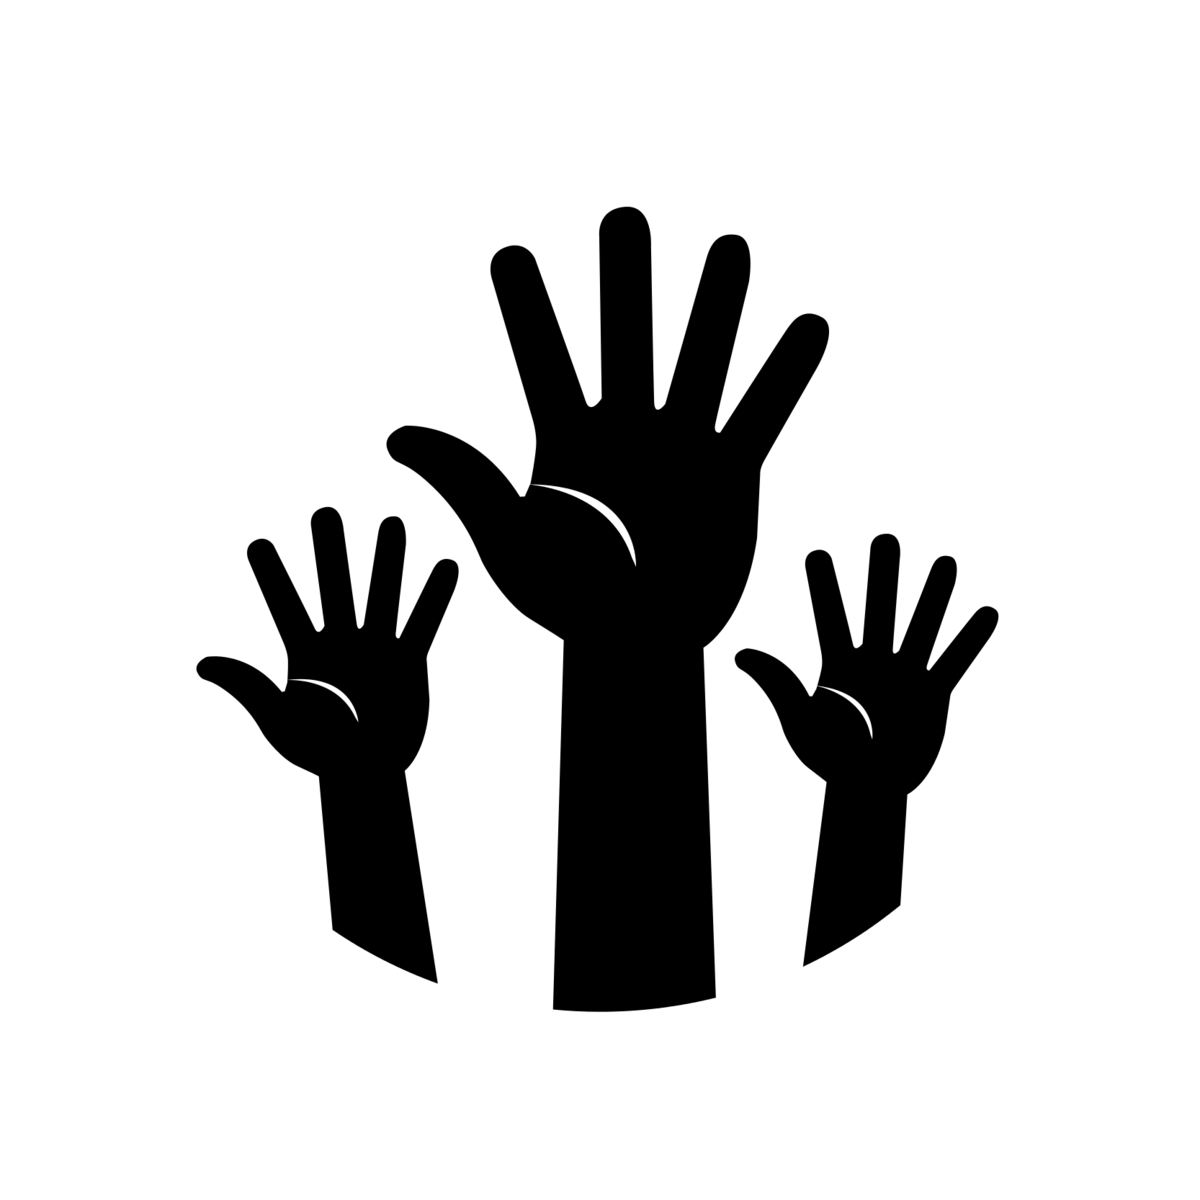
\includegraphics[height=0.5cm]{images/hands.png}\\
\pause
$\to$ use penalized runtime scores (PAR$10$)

\end{frame}
%-----------------------------------------------------------------------
%----------------------------------------------------------------------
\begin{frame}[c]{\satzillaY{11}: toy example voting}

For a given instance $\inst$ and for each pair of algorithms $(\algo_i, \algo_j)$, 
predict whether $\algo_i$ will perform better than $\algo_j$ on $\inst$.

\bigskip

\[
\begin{array}{| r | c  c  c || c |}
  \cline{1-5}
   Pred.   & \algo_1 & \algo_2 & \algo_3 & votes\\
  \cline{1-5}
  \algo_1 &      & 1  &  0  & 1\\
  \algo_2 &  0    &   &  0  & 0\\
  \algo_3 &  1    & 1  &    & 2\\
  \cline{1-5}
\end{array}
\]

\pause
\begin{center}
$\to$ select $\algo_3$ 
\end{center}

\bigskip
\pause

Tie-breaker: better average performance on training.

\end{frame}
%-----------------------------------------------------------------------
%----------------------------------------------------------------------
\begin{frame}[c]{Pairwise Regression Models}

\begin{block}{Intuition}
\begin{itemize}
  \item \satzilla{}'09 trains an performance model for each algorithm to predict its (log) runtime
  \pause
  \item We are not interested in the performances of each algorithms, but in a ranking of the algorithms
  \item Pairwise regression models \lit{L. Kotthoff, LLAMA 2013} to predict the performance differences and rank the algorithms accordingly
\end{itemize}
\end{block}

\pause

\begin{block}{Implementation}
  \begin{enumerate}
    \item For each pair of algorithms $(\algo_1, \algo_2)$, predict the performance difference between them $\delta(\algo_1, \algo_2)$ 
    \item Score each algorithm by the sum of its performance differences $\text{score}(\algo) = \sum_{\algo' \in \portfolio} \delta(\algo, \algo')$
    \item Select the algorithm with the smallest score
  \end{enumerate}
\end{block}

\end{frame}
%-----------------------------------------------------------------------
%----------------------------------------------------------------------
\begin{frame}[c]{Pairwise Regression Models - Toy Example}

Training:
\[
\begin{array}{| r | c  c  || c |}
  \cline{1-4}
      & \algo_1 & \algo_2 & y = \algo_1 - \algo_2\\
  \cline{1-4}
  \inst_1 & 		 1    &         10  &  -9 \\
  \inst_2 &          5    &         10  &  -5\\
  \inst_3 &          8    &  		1   & 7\\
  \inst_4 &         10  &           10  & 0\\
  \inst_5 &         10  & 		    6   & 4\\
  \inst_6 &         10  &           8   & 2\\
  \cline{1-4}
\end{array}
\]

\pause

Selection:
\[
\begin{array}{| r | c  c  c || c |}
  \cline{1-5}
  Pred.    & \algo_1 & \algo_2 & \algo_3 & Scores\\
  \cline{1-5}
  \algo_1 &      & -2  &  4  & 2\\
  \algo_2 &  2    &   &  6  & 8\\
  \algo_3 &  -4    & -6  &    & -10\\
  \cline{1-5}
\end{array}
\]

\centering
$\to$ run $\algo_3$

\end{frame}
%-----------------------------------------------------------------------
%----------------------------------------------------------------------
\begin{frame}[c]{Instance-Specific Algorithm Configuration: \isac{}\\ \litw{S. Kadioglu et al. 2010}}

\begin{block}{Intuition}
\begin{itemize}
  \item (Training) instances can be partitioned in homogeneous subsets
  \item Each homogeneous subset can be assigned to a well-performing algorithm
\end{itemize}
\end{block}

\pause

\begin{block}{Approach - Training}
\begin{enumerate}
  \item Cluster the training instances into homogeneous subsets $\clusters$ \\ (using g-means~\lit{Hamerly and Elkan 2003})
  \item Assign the best performing algorithm to each $\cluster \in \clusters$ 
\end{enumerate}
\end{block}

\pause

\begin{block}{Approach - Selection}
\begin{enumerate}
  \item For a new instance, compute the cluster $\cluster \in \clusters$ it belongs to
  \item Select the algorithm of $\cluster$
\end{enumerate}
\end{block}

\end{frame}
%-----------------------------------------------------------------------
%----------------------------------------------------------------------
\begin{frame}[c]{Instance-Specific Algorithm Configuration: \isac{}\\ \litw{S. Kadioglu et al. 2010}}

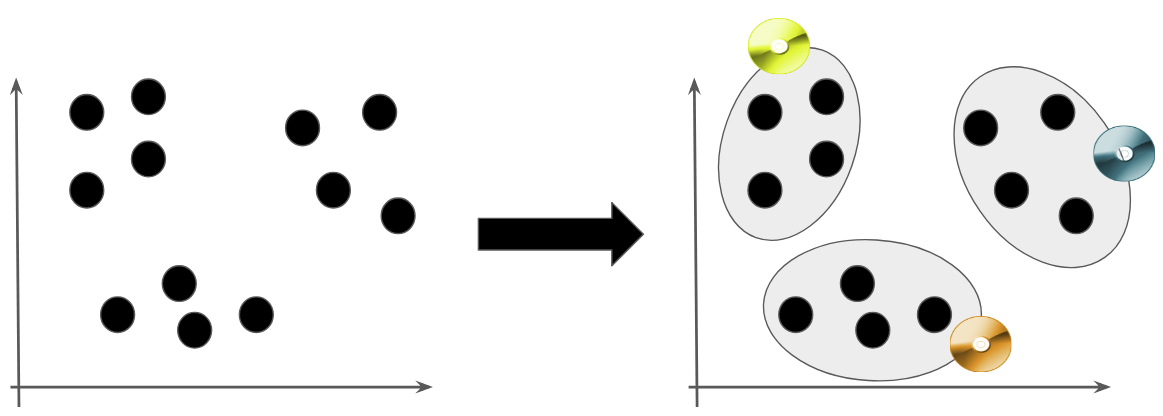
\includegraphics[width=0.9\textwidth]{images/isac}

\end{frame}
%-----------------------------------------------------------------------
%----------------------------------------------------------------------
\begin{frame}[c]{Cost-Sensitive Hierarchical Clustering: \cshc{}\\ \litw{Y. Malitsky et al. 2013}}

\begin{block}{Problems of \isac{}}
\begin{itemize}
  \item \isac{} uses unsupervised learning (i.e., clustering)
  \begin{itemize}
    \item Sensitive to feature scaling
    \item Which distance metric in feature space?
    \item We cannot assess the quality of the clusters
  \end{itemize}
  \item[$\to$] \cshc{} partition the instances by looking at performance data
\end{itemize}
\end{block}


\begin{block}{Approach - Training}
\begin{enumerate}
  \item Train a decision tree such that each leaf maximally agrees on the best-performing algorithm $\to$ homogeneous instance sets
  \item Uses bagging to further improve performance (as in random forests)
\end{enumerate}
\end{block}


\end{frame}
%-----------------------------------------------------------------------
%----------------------------------------------------------------------
\begin{frame}[c]{Cost-Sensitive Hierarchical Clustering: \cshc{}\\ \litw{Y. Malitsky et al. 2013}}

\centering
\includegraphics[width=0.5\textwidth]{images/csch_tree}

\end{frame}
%-----------------------------------------------------------------------
%----------------------------------------------------------------------
\begin{frame}[c]{Cost-Sensitive Hierarchical Clustering: \cshc{}\\ \litw{Y. Malitsky et al. 2013}}


\begin{block}{Homogeneity Metric}
\begin{equation}
h(\insts) = \underbrace{\min_{\algo \in \portfolio} \sum_{\inst \in \insts} c(\algo, \inst)}_{\text{single best}} - \underbrace{\sum_{\inst \in \insts} \min_{\algo \in \portfolio} c(\algo, \inst)}_{oracle} \nonumber
\end{equation}
\end{block}

\pause

\begin{block}{Split Criterion}
Find a split of $\insts$ into $\hat{\insts}_1$ and $\hat{\insts}_2$ such that:
\begin{equation}
(\hat{\insts}_1,\hat{\insts}_2) \in \argmin_{\insts_1 \cup \insts_2 = \insts} h(\insts_1) + h(\insts_2)\nonumber
\end{equation}
\end{block}

\end{frame}
%-----------------------------------------------------------------------
% %----------------------------------------------------------------------
% \begin{frame}[c]{\cshc{} - Example}
% 
% 
% 
% \end{frame}
% %-----------------------------------------------------------------------
% %----------------------------------------------------------------------
% \begin{frame}[c]{\sss~\litw{S. Kadioglu et al. 2011}}
% 
% \begin{block}{Idea}
% \begin{itemize}
%   \item Similar instances in the feature space have the same well-performing algorithms
% \end{itemize}
% \end{block}
% 
% \pause
% 
% \begin{block}{Training}
% \begin{itemize}
%   \item Compute a timeout-minimal pre-solving algorithm schedule
%   \item Train selector based on $k$-NN
%   \begin{itemize}
%     \item distance-based weighting
%     \item clustering-based adaptive neighborhood size (see Lecture 4 on ML)
%   \end{itemize}
% \end{itemize}
% \end{block}
% 
% \pause
% 
% \begin{block}{Selection}
% \begin{enumerate}
%   \item For $10\%$ of the runtime cutoff, run pre-solving schedule 
%   \item Determine the $k$ most similar instances $\insts_k$ in the feature space
%   \item Select the algorithm with the best (training) performance on $\insts_k$
% \end{enumerate}
% \end{block}
% 
% \end{frame}
% %-----------------------------------------------------------------------
%----------------------------------------------------------------------
\begin{frame}[c]{\sunny~\litw{R. Amadini et al. 2014}}

\begin{block}{Idea}
\begin{itemize}
  \item Selectors are imperfect
  \item Select a schedule of algorithms to improve robustness
\end{itemize}
\end{block}

\pause

\begin{block}{Training}
Essentially none
\end{block}

\pause

\begin{block}{Selection}
\begin{enumerate}
  \item Use $k$-NN in feature space\\ to select $k$ most similar training instances
  \pause
  \item Each $\algo$ gets a time slot for each instance it can solve
  \pause
  \item Backup algorithm gets a time slot for each unsolved instance
  \pause
  \item Normalize time slots for available time budget
  \pause
  \item Sort algorithms by their average PAR10 score,\\
  		i.e., most promising algorithm first
\end{enumerate}
\end{block}

\end{frame}
%-----------------------------------------------------------------------
%----------------------------------------------------------------------
\begin{frame}[c]{On-going Evaluation of Algorithm Selectors}

\small
\begin{table}
\begin{tabular}{l | cc | c c c c}
\toprule
Scenario & Oracle & SB & aspeed & ISAC & SATzilla'14 & LLAMA\\
\midrule
ASP & 21.3 & 534.1 & 353.3 & 291.9 & 170.0 & \textbf{137.6}\\
OR & 227.6 & 7,002.9 & \textbf{1,964.1} & 5,880.8 & 3,179.1 & 5,546.5\\
SAT12-INDU & 88.1 & 1,360.6 & 1,645.4 & 1,409.5 & 839.7 & \textbf{783.4}\\
SAT12-RAND & 46.9 & 568.5 & 713.9 & \textbf{434.5} & 485.3 & 527.0\\
\bottomrule
\end{tabular}
\end{table}

\centering
\small
All results on \url{aslib.net}

\bigskip
\pause
\begin{itemize}
  \item The best algorithm selection approach depends on the application.
  \item On average, \satzilla{} (with cost-sensitive classification) performs well 
\end{itemize}


\end{frame}
%-----------------------------------------------------------------------
%----------------------------------------------------------------------
\begin{frame}[c]{Bells and Whistles in Algorithm Selection}

\begin{columns}
	\begin{column}{0.45\textwidth}
		\begin{block}{Feature Preprocessing}
		\begin{itemize}
		  \item normalization
		  \begin{itemize}
		    \item standard scaling
		    \item linear scaling
		    \item log scaling
		  \end{itemize}
		  \item feature selection, PCA
		  \item missing features imputation
		  \item max time to compute features
		\end{itemize}
		\end{block}
	\end{column}
	\begin{column}{0.45\textwidth}
		\begin{block}{Performance Preprocessing}
		\begin{itemize}
		  \item transformation:\\ log or z-score
		  \item instance weighting
		  \item algorithm filtering
		\end{itemize}
		\end{block}
		\begin{block}{Pre-Solving}
			\begin{itemize}
			  \item how many algorithms?
			  \item how long?
			\end{itemize}
		\end{block}
	\end{column}

\end{columns}


\bigskip
\pause

$\leadsto$ Besides choosing the right algorithm selection approach,\\
you have to choose further techniques.

\pause

$\leadsto$ Everything has (hyper-) parameters.

\end{frame}
%-----------------------------------------------------------------------
%----------------------------------------------------------------------
\begin{frame}[c]{\flexfolio~\litw{Lindauer et al. 2015: \autofolio}}

\scalebox{0.57}{
\begin{tikzpicture}[node distance=0.6cm]
	%PreProcessing
	\pause
	\node (Instance) [data] {Training\\ Instances};
	\node (Solvers) [data, right=of Instance] {Portfolio};
	\node (Runtimes) [activity, below=of Solvers, text width = 9em, yshift=-1.6em] {Assess\\ Performance};
	\node (Features) [activity, below=of Instance, text width = 9em, yshift=-1.3em] {Compute Features};
	\node (claspre) [data, left=of Features] {Feature Generator};
	
	
	\draw[myarrow] (Instance) -- (Runtimes.north west);
	\draw[myarrow] (Instance) -- (Features.north);
	\draw[myarrow] (Solvers) -- (Runtimes.north);
	\draw[myarrow] (claspre) -- (Features);
	
	\pause
	% Training Model
	\node (FeatPre) [activity, below=of Features, text width = 9em, yshift=-2em] {Feature\\ Preprocessing};
	\node (TimePre) [activity, below=of Runtimes, text width = 9em, yshift=-1.3em] {Performance Preprocessing};
	\node (Training) [activity, below=of TimePre, text width = 10em, yshift=-0.4em] {Train Selection Model};
	\draw[myarrow] (Runtimes) -- (TimePre);
	\draw[myarrow] (Features) -- (FeatPre);
	\draw[myarrow] (TimePre) -- (Training);
	\draw[myarrow] (FeatPre) |- (Training);
	
	\pause
	%CV
	\node (CVML) [activity, right=of TimePre, text width = 11em, xshift=1em] {Performance Estimation};
	\node (Aspeed) [activity, below=of CVML, text width = 9em, yshift=-0.5em] {Algorithm Schedule\\ by \aspeed};

	\draw[myarrow, bend left=20] (Runtimes) |- ++(8.00,0.0) |- (Aspeed);
	\draw[myarrow] (CVML) -- (Aspeed);
	\draw[myarrow, dashed, shorten <=0.43cm] (TimePre) -- node [above] {} (CVML);
	
	\pause
    \draw[myarrow, dashed] (Aspeed) -- node [above, pos=0.5, font=\tiny] {Feedback} (Training);
	
	\pause	
	\node (RunSBS) [activity, below=of Aspeed, text width=10em, yshift=-3.0em] {Optimize and Run\\ Pre-Solving Schedule};
	\node (Run) [activity, right=of RunSBS, xshift=0.5cm] {Run Selected Algorithm};
	
	
	\draw[myarrow] (Aspeed) -- (RunSBS);
	\draw[myarrow] (RunSBS) -- node [above] {failed} (Run);
	
	% Run new Instance
	\node (Predict) [activity, left=of RunSBS, xshift=0.0em] {Select Algorithm};
	\node (TestFeatures) [activity, left=of Predict] {Compute Features};
	\node (TestInstance) [data, left=of TestFeatures] {(New) Instance};
	%\node (Backup) [activity, below=of TestFeatures] {Run Backup Algorithm};
	
	\draw[myarrow] (Training.south) -- ($(Predict.north)+(-0.76,0.0)$);
	\draw[myarrow] (TestInstance) -- (TestFeatures);
	\draw[myarrow] (TestFeatures) -- (Predict.west);
	\draw[myarrow] (Predict) -- (RunSBS.west);
	%\draw[myarrow] (TestFeatures) -- node [left] {failed} (Backup);		
	\draw[myarrow] (claspre.south) -- ($(TestInstance.north)+(-1.0,0.55)$) -| (TestFeatures.north);	
	
    \begin{pgfonlayer}{background}
    
        % Ressources
    	%\path (Instance -| Instance.west)+(-0.25,0.55) node (resUL) {};
    	%\path (Solvers.east |- Solvers.south)+(0.75,-0.5) node(resBR) {};
    	%\path [rounded corners, draw=black!60, dashed] (resUL) rectangle (resBR);
		%\path (Solvers.east |- Solvers.south)+(-0.2,-0.3) node [text=black!60] {Resources};
    
        % Data Collection
    	\path (Instance -| Instance.west)+(-0.35,0.65) node (dataUL) {};
    	\path (Runtimes.east |- Runtimes.south)+(1.05,-0.5) node(dataBR) {};
    	\path [rounded corners, draw=black!60, dashed] (dataUL) rectangle (dataBR);
		\path (Runtimes.east |- Runtimes.south)+(-0.35,-0.3) node [text=black!60] {Training Data};
    	
    	% Prediction
    	\path (TimePre -| FeatPre.west)+(-0.25,0.65) node (trainUL) {};
    	\path (Training.east |- Aspeed.south)+(0.25,-0.5) node(trainBR) {};
    	\path [rounded corners, draw=black!60, dashed] (trainUL) rectangle (trainBR);
    	\path (Training.east |- Aspeed.south)+(-0.75,-0.3) node [text=black!60] {Selection};
    	
    	% Aspeed Training
    	\path (CVML -| CVML.west)+(-0.25,0.65) node (trainUL) {};
    	\path (CVML.east |- Aspeed.south)+(0.25,-0.5) node(trainBR) {};
    	\path [rounded corners, draw=black!60, dashed] (trainUL) rectangle (trainBR);
    	\path (Aspeed.east |- Aspeed.south)+(-0.4,-0.3) node [text=black!60] {Scheduling};
    	
    	% Training
    	\path (CVML -| FeatPre.west)+(-0.5,0.85) node (trainUL) {};
    	\path (CVML.east |- Aspeed.south)+(1.0,-1.1) node(trainBR) {};
    	\path [rounded corners, draw=black!60, dashed] (trainUL) rectangle (trainBR);
    	\path (Aspeed.east |- Aspeed.south)+(0.55,-0.9) node [text=black!60] {Training};
    	
    	%Test
    	\path (TestFeatures.west)+(-0.2,0.65) node (testUL) {};
    	\path (Run.east |- Run.south)+(0.2,-0.5) node(testBR) {};
    	\path [rounded corners, draw=black!60, dashed] (testUL) rectangle (testBR);
    	\path (Run.east |- Run.south)+(-0.6,-0.3) node [text=black!60] {Solving};
    	
    \end{pgfonlayer}
    
\end{tikzpicture}
}

\end{frame}
%-----------------------------------------------------------------------
% %----------------------------------------------------------------------
% \begin{frame}[c]{Approaches~\litw{Lindauer et al. 2015: \autofolio}}
% 
% \scalebox{0.4}{
% 
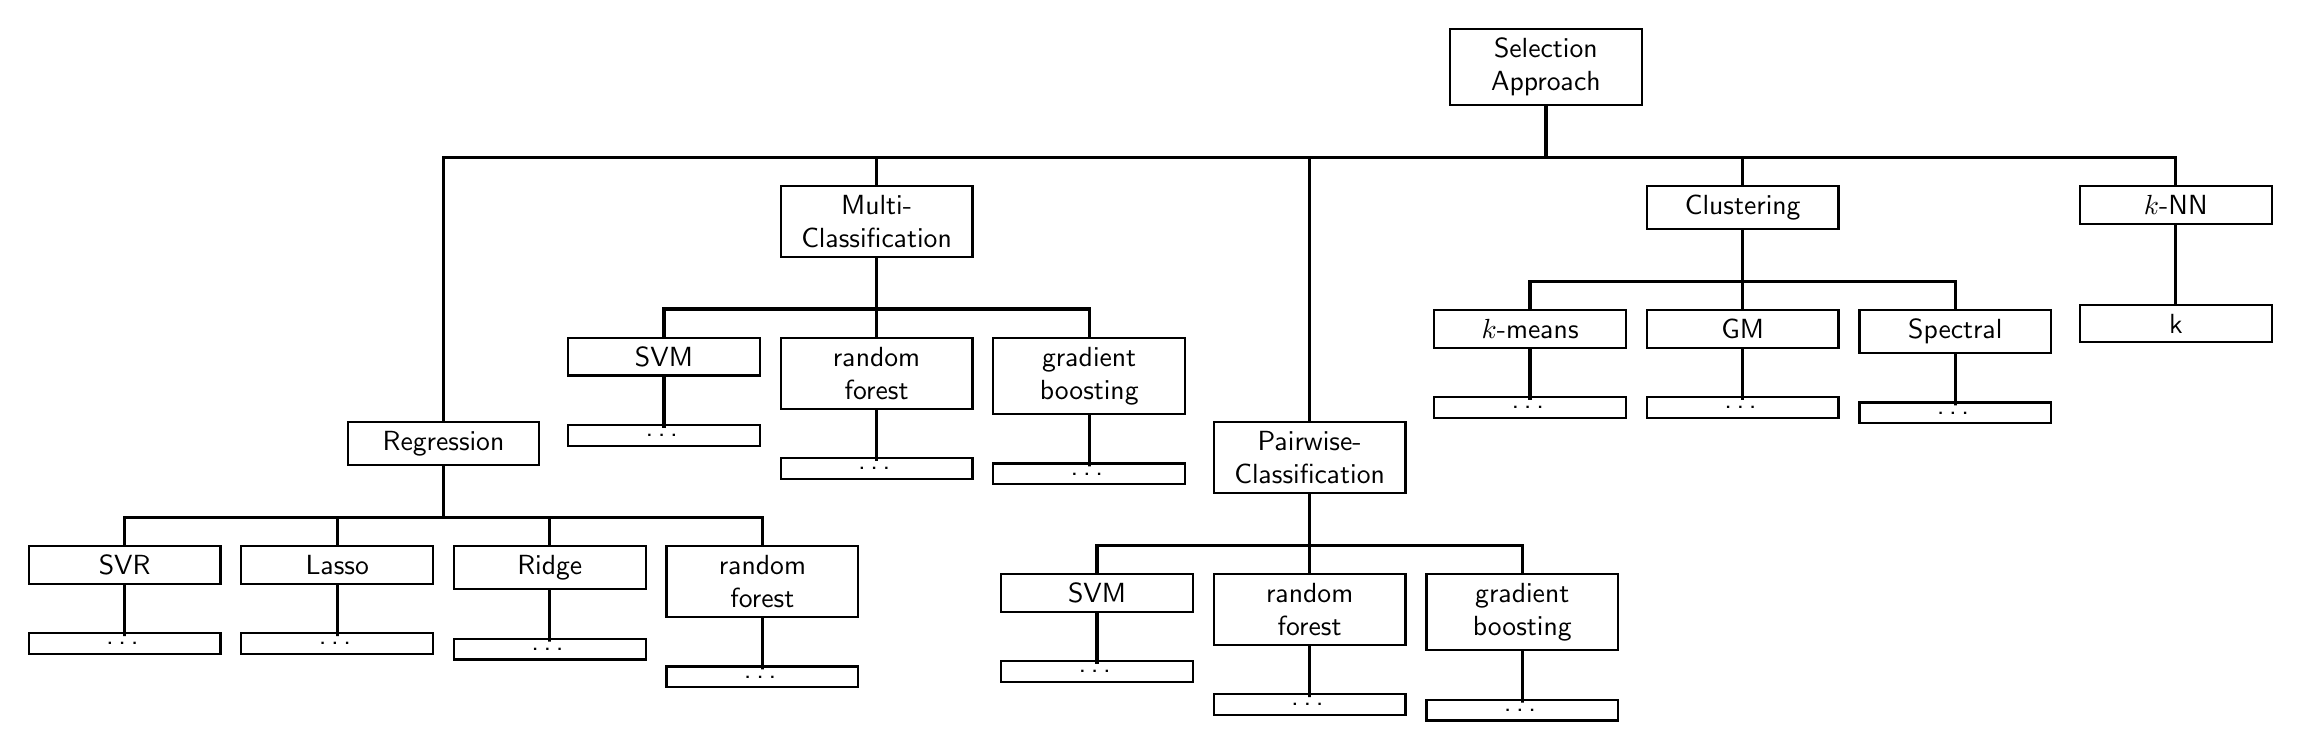
\begin{tikzpicture}[
% Label style
    label distance=3mm,
    every label/.style={blue},
% Event style
    event/.style={rectangle,thick,draw,text width=2.2cm,
		text centered,font=\sffamily,anchor=north},
% Children and edges style
    edge from parent/.style={very thick,draw=black},
    edge from parent path={(\tikzparentnode.south) -- ++(0,-.65cm) -| (\tikzchildnode.north)},
	level 1/.style={sibling distance=7cm, level distance=1.0cm, growth parent anchor=south,nodes=event},
    level 2/.style={sibling distance=6.0cm, level distance=1.0cm},
    level 3/.style={sibling distance=2.4cm,level distance=0.6cm},
    %level 4/.style={sibling distance=5cm},
    %level 5/.style={sibling distance=5cm}
    %level 6/.style={sibling distance=6cm}
%%  For compatability with PGF CVS add the absolute option:
%   absolute
    ]
%% Draw events and edges
    \node (comp) [event] {Selection Approach} 
       child{
       	  node [sibling distance=8.9cm, yshift=-3.0cm] {Regression}
       	  child [sibling distance=2.7cm] {
				node {SVR}
				child { node {\ldots}}	
		  }				       	  
  		  child [sibling distance=2.7cm] {
  				node {Lasso}   
  				child { node {\ldots}}	
	       }
	      child [sibling distance=2.7cm] {
  				node {Ridge}   
  				child { node {\ldots}}	
	       } 
	       child [sibling distance=2.7cm] {
  				node {random\\ forest}  
  				child { node {\ldots}}	 
	       } 
       }
        child{
       	  node [sibling distance=8.9cm, xshift=-1.5cm]  {Multi-Classification}
       	  child [sibling distance=2.7cm] {
				node  {SVM}
				child { node {\ldots}}	
		  }				       	  
  		  child [sibling distance=2.7cm] {
  				node {random\\ forest}   
  				child { node {\ldots}}	
	       }
	      child [sibling distance=2.7cm] {
  				node {gradient boosting}   
  				child { node {\ldots}}	
	       }
	     } 
	     child{
       	  node [sibling distance=8.9cm, yshift=-3.0cm, xshift=-3.0cm] {Pairwise-Classification}
       	  child [sibling distance=2.7cm] {
				node  {SVM}
				child { node {\ldots}}	
		  }				       	  
  		  child [sibling distance=2.7cm] {
  				node {random\\ forest}   
  				child { node {\ldots}}	
	       }
	      child [sibling distance=2.7cm] {
  				node {gradient boosting}   
  				child { node {\ldots}}	
	       }
	      }
	      child{
       	  node [sibling distance=8.9cm, xshift=-4.5cm] {Clustering}
       	  child [sibling distance=2.7cm] {
				node {$k$-means}
				child { node {\ldots}}	
		  }				       	  
  		  child [sibling distance=2.7cm] {
  				node {GM}   
  				child { node {\ldots}}	
	       }
	      child [sibling distance=2.7cm] {
  				node {Spectral}   
  				child { node {\ldots}}	
	       }
	      } 
	      child{
       	  node [sibling distance=8.9cm, xshift=-6.0cm] {$k$-NN}
       	  child [sibling distance=2.7cm] {
				node  {k}
		  	}
       };
	     
\end{tikzpicture}

% }
% 
% \end{frame}
% %-----------------------------------------------------------------------
%----------------------------------------------------------------------
\begin{frame}[c]{How to assess the performance of algorithm selectors?}

Issues with old AS papers:

\begin{enumerate}
  \item Tedious and time-consuming task to collect data for more than $2-3$ scenarios\\ $\leadsto$ only few experimental results
	\pause
  \medskip
  \item Everyone uses other scenarios\\ $\leadsto$ incomparable results
  \item Runtimes are measured on different hardware\\ $\leadsto$ incomparable results
  \pause
  \medskip
  \item Scenarios are not always publicly available\\ $\leadsto$ incomparable results
  \pause
  \medskip
  \item Beginners (and even experts) make mistakes\\ e.g., don't consider feature costs \\ $\leadsto$ invalid results
\end{enumerate}
\end{frame}
%-----------------------------------------------------------------------
%----------------------------------------------------------------------
\begin{frame}[c]{How to assess the performance of algorithm selectors?}

\begin{block}{Fair Comparison}
Algorithm selectors get the same input:
\begin{itemize}
  \item algorithm portfolio $\portfolio$
  \item training instances $\insts$
  \item instance features $\feats$
\end{itemize}
\end{block}

\begin{block}{ASlib (Algorithm Selection Library)}
ASlib provides:
\begin{itemize}
  \item performance of each algorithm on each instance: $c(\algo,\inst)$
  \item instance features of each instance: $\feat(\inst)$
  \item cost to compute instance features
\end{itemize}
\end{block}

\end{frame}
%-----------------------------------------------------------------------
%----------------------------------------------------------------------
\begin{frame}[c]{ASlib $v.1.0$ Scenarios}

\centering

\small
\begin{tabular}{l ccccccc}
\hline
\hline
Scenario 				& $|I|$ &		$|A|$ 		& $\# f$  	& $\varnothing t_f$ & Ref.\\
\hline
\aspCoseal 	 			& $1294$			& $11$ 	 		& $138$ 	 & $1.3$ 	& \lit{Hoos et al. 2014} \\
\pause
\cspCoseal  	 		& $2024$			& $2$ 	 		& $17$  	& $n/a$ 		& \lit{Gent et al. 2010}	 \\
\maxsatCoseal 			& $876$				& $6$ 	 		& $37$  	& $0.1$	& \lit{Ansotegui et a. 2014} \\
\premarCoseal 			& $527$ 			& $4$ 			& $16$		 & $n/a$ & \lit{Tierney et al. 2014}\\
\proteusCoseal			& $4021$			& $22$			& $198$		 & $6.4$  & \lit{Hurley et al. 2014}\\
\qbfCoseal 	 			& $1368$			& $5$ 	 		& $46$  	 & $n/a$ 	& \lit{Kotthoff et al. 2012}\\
\sathandElevenCoseal 	& $296$ 	 		& $15$ 	 		& $115$  	 & $41.2$ 	& \lit{Xu et al. 2012}\\
\satinduElevenCoseal 	& $300$				& $18$ 	 		& $115$  	 & $135.3$ 	& \lit{Xu et al. 2012} \\
\satrandElevenCoseal 	& $600$ 			& $9$ 	 		& $115$  	 & $22.0$	& \lit{Xu et al. 2012} \\
\satallTwelveCoseal		& $1614$			& $31$ 	 		& $115$		 & $40.5$  & \lit{Xu et al. 2012} \\
\sathandTwelveCoseal 	& $767$				& $31$ 	 		& $115$  	 & $39.0$  & \lit{Xu et al. 2012} \\
\satinduTwelveCoseal  	& $1167$			& $31$ 	 		& $115$  	 & $80.9$  & \lit{Xu et al. 2012} \\
\satrandTwelveCoseal  	& $1362$			& $31$ 	 		& $115$ 	 & $9.0$ & \lit{Xu et al. 2012} \\
\hline
\hline
\end{tabular}
 
\medskip
(ASlib $v.4.0$ has $29$ scenarios.)

\bigskip
\pause

\end{frame}
%-----------------------------------------------------------------------
%----------------------------------------------------------------------
\begin{frame}[c]{ASlib Scenarios}

\centering
\begin{tabular}{c c}
\hline
\hline
Scenario & Data Collection Time (\textbf{CPU Days})\\
\hline
\aspCoseal & $25$\\
\pause
\premarCoseal  & $28$\\
\cspCoseal & $52$\\
\maxsatCoseal & $56$\\
\pause
\satinduElevenCoseal & $128$\\
\satrandElevenCoseal & $158$\\
\qbfCoseal & $163$\\
\sathandElevenCoseal & $168$\\
\pause
\sathandTwelveCoseal & $234$\\
\satinduTwelveCoseal & $284$\\
\pause
\satallTwelveCoseal & $415$\\
\satrandTwelveCoseal & $447$\\
\proteusCoseal & $596$\\
\hline
\hline
\end{tabular}

\bigskip
\pause
$\leadsto$ Gathering of training data can be crazy expensive.

\end{frame}
%-----------------------------------------------------------------------
%----------------------------------------------------------------------
\begin{frame}[c]{Cons of ASlib}

\begin{itemize}
  \item Performance of algorithm can depend on hardware
  \medskip
  \pause
  \item Feature construction is part of algorithm selection
  \begin{itemize}
    \item Lorregia et al. '16 proposed to use deep learning to learn features from text representation
  \end{itemize}
  \medskip
  \pause
  \item Algorithm design is part of algorithm selection
  \begin{itemize}
    \item Parameter configuration of each algorithm
  \end{itemize}
\end{itemize}

\bigskip
\pause
$\leadsto$ You can use ASlib ``only'' to compare selection approaches.

\end{frame}
%-----------------------------------------------------------------------
% %----------------------------------------------------------------------
% \begin{frame}[c]{When to apply Algorithm Selection?}
% 
% \centering
% \scalebox{0.7}{
% \begin{tikzpicture}[
% Label style
    thick,
    label distance=3mm,
    every label/.style={blue},
% Event style
    event/.style={rectangle,thick,draw,text width=2.2cm,
		text centered,font=\sffamily,anchor=north},
% Children and edges style
    edge from parent/.style={very thick,draw=black},
    edge from parent path={(\tikzparentnode.south) -- ++(0,-.65cm)
			-| (\tikzchildnode.north)},
	level 1/.style={sibling distance=7cm,level distance=1.0cm,
			growth parent anchor=south,nodes=event},
    level 2/.style={sibling distance=6.0cm,level distance=1.0cm},
    level 3/.style={sibling distance=3.4cm,level distance=1.0cm},
    level 4/.style={sibling distance=5cm},
    level 5/.style={sibling distance=5cm}
    level 6/.style={sibling distance=6cm}
%%  For compatability with PGF CVS add the absolute option:
%   absolute
    ]
%% Draw events and edges
    \node (comp) [event] {Instance Distribution?} 
       child{
       	  node [sibling distance=1.9cm] (par1) {Parallel Solving?}
       	  child [sibling distance=2.7cm] {
				node (conf) {Algorithm Configuration} 
		  }				       	  
  		  child [sibling distance=2.7cm] {
  				node (apps) {Conf. Par. Portfolios}   
	       }
       }
       	  child {
	      	node (feat) {Instance Features?}
			     child{
			     	node [] (par2) {Parallel Solving?}    
			     		child{
			     			node [text width=2.9cm] (saspeed) {Optimized\\ Sequential\\ Schedules}
			     		}
			     		child{
			     			node [text width=2.4cm] (paspeed) {Optimized\\ Parallel Schedules} 
			     		}
					}
				child{
			     	node [] (par3) {Parallel Solving?}    
			     		child{
			     			node [text width=2.1cm] (cf) {Algorithm Selection}
			     		}
			     		child{
			     			node [text width=3.3cm] (cfpasu) {Parallel Portfolio\\ Selection} 
			     		}
					}
	 	};	
	     
	\node	at ($(par1.north)+(0,0.7)$) {homogeneous};
	\node	at ($(feat.north)+(0,0.7)$) {heterogeneous};
	\node	at ($(conf.north)+(0,0.7)$) {no};
	\node	at ($(apps.north)+(0,0.7)$) {yes};	     
	\node	at ($(par2.north)+(0,0.7)$) {not available};
	\node	at ($(par3.north)+(0,0.7)$) {available};
	\node	at ($(saspeed.north)+(0,0.7)$) {no};
	\node	at ($(paspeed.north)+(0,0.7)$) {yes};
	\node	at ($(cf.north)+(0,0.7)$) {no};
	\node	at ($(cfpasu.north)+(0,0.7)$) {yes};
\end{tikzpicture}	
% }
% 
% \end{frame}
% %-----------------------------------------------------------------------
%----------------------------------------------------------------------
\begin{frame}[c]{When to apply Algorithm Selection?}

\begin{enumerate}
  \item The performance of your algorithms is \alert{complementary}
  \begin{itemize}
    \item instead of a set of algorithms, you can also use\\ a finite set of different parameter configurations of one algorihtm.
  \end{itemize}
  \pause
  \item Your instances are \alert{heterogeneous}
  \begin{itemize}
    \item[$\to$] for different instances, different algorithms perform well
  \end{itemize}
  \pause
  \item Your instances can be described by \alert{informative instance features}
  \begin{itemize}
    \item That's actually a big issue for meta-features of machine learning datasets
  \end{itemize}
  \pause
  \item Your instance features can be \alert{computed in a reasonable time.}
  \begin{itemize}
    \item the time to compute the features should be much smaller\\ than the time required to apply an algorithm to an instance
  \end{itemize}
  \item You can gather sufficient \alert{training data}\\ to train your selection model(s)
  \begin{itemize}
    \item Typically that requires a compute cluster
  \end{itemize}
\end{enumerate}

\pause
$\leadsto$ \alert{If all these apply, you can train efficient algorithm selectors
and\\ improve the performance of your system substantially.}

\end{frame}
%-----------------------------------------------------------------------
%----------------------------------------------------------------------
\begin{frame}[c]{Literature}

\begin{itemize}
  \item \lit{L. Xu, F. Hutter, H. H. Hoos, K. Leyton-Brown. SATzilla: Portfolio-based Algorithm Selection for SAT. In: Journal of Artificial Intelligence Research, Volume 32, pp. 565–606, 2008}
  \item \lit{Lars Kotthoff. Algorithm Selection for Combinatorial Search Problems: A Survey. In: AI Magazine, 2014}
  \item Literature overview: \url{http://larskotthoff.github.io/assurvey/}
  \item How to handle the (hyper-)parameters in algorithm selection:\\
  \lit{M. Lindauer and H. Hoos and F. Hutter and T. Schaub. AutoFolio: An automatically configured Algorithm Selector. In: Journal of Artificial Intelligence 53 (2015): 745-778} 
\end{itemize}



\end{frame}
%-----------------------------------------------------------------------
%----------------------------------------------------------------------
\begin{frame}[c]{Learning Goals}

After this lecture, you will be able to \ldots

\begin{itemize}
  \item explain all components of \alert{\satzilla}
  \item explain other algorithm selection approaches
  \begin{itemize}
	  \item \alert{pair-wise regression} 
	  \item \alert{cost-sensitive classification} 
	  \item \alert{clustering} 
	  \item \alert{kNN}
	  \item \alert{per-instance algorithm schedules}
  \end{itemize}
  \item describe a \alert{flexible framework} for algorithm selection
  \item decide \alert{when} to use algorithm selection
  %\item combine of \alert{algorithm selection and configuration}
\end{itemize}

\end{frame}
%-----------------------------------------------------------------------